\subsection*{research}
i discovered \autocite{rf-amp-classics} (see \localfile{../research/books/}),
an \arrl book on \rf amplifiers, and skimmed through it. some items of
interest:
\begin{enumerate}
	\item \autocite[p.~1 dash 41]{rf-amp-classics}: class-E power
	amplifiers are a highly power- and parts-efficient amplifier topology,
	utilizing a single active element and a tuned load. the article,
	``High-Efficiency Class-E Power Amplifiers,'' claims 21-fold power
	improvement over class-A for a given dissipated power. since our
	fractional bandwidth is not that high (\textasciitilde 2.5 \%), we
	could get away with a Q of 40 in the tuned load and still transmit
	across the band, so class-E might be feasible! the circuit used in the
	article is reproduced in figure \ref{fig:class-e-from-article}.

	\begin{figure}[H]
		\centering
		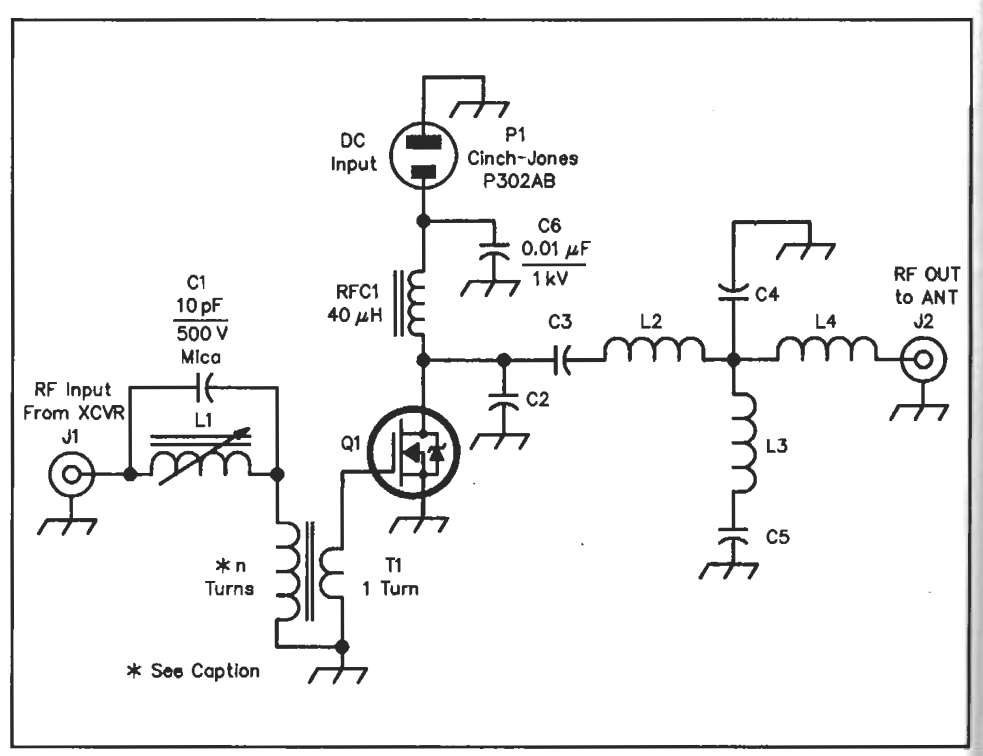
\includegraphics[width=.7\textwidth]{class-e-from-article.png}
		\caption{a class-E amplifier.}
		\label{fig:class-e-from-article}
	\end{figure}

	i have a slight advantage in that i know about these amplifiers from
	elsewhere\ldots\ but here's how they work anyway: the load network
	comprising C2, C3, C4, C5, L2, L3, \amp L4 (basically everything
	hanging off Q1's drain) is resonant somewhere near the transmission
	frequency. the network is carefully damped, so that when Q1 switches
	off, the voltage across it rises, then neatly falls back to zero just
	by the next turn-on. figure \ref{fig:class-e-vi}, also from the
	article, shows this.

	\begin{figure}[H]
		\centering
		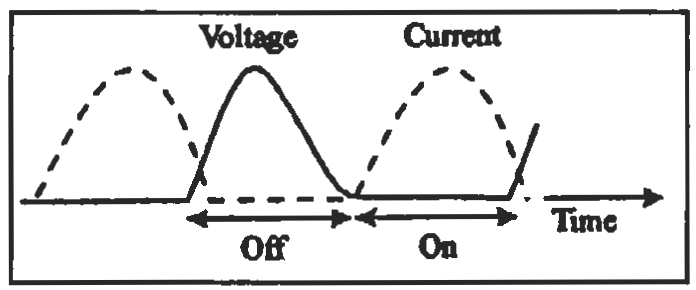
\includegraphics[width=.7\textwidth]{class-e-vi.png}
		\caption{class-E voltage \amp current.}
		\label{fig:class-e-vi}
	\end{figure}

\end{enumerate}

\subsection*{code}
i typeset this log and wrote the first two entries.
